\section{Elementary Geometry}
Elementary geometry is about basic geometric features of basic shapes in the 2D plane or 3D space such as lengths, areas, volumes, angles, etc. of triangles, quadrilaterals, circles etc.. It's mostly a catalog of laws, formulas or algorithms to compute quantities of interest given some other quantities. For example, if we know two angles of a triangle, there's a simple formula to compute the third. If we know the length of a side and the height above that side in a triangle and we want to know the area of the triangle, there's a formula for that, too. If we know the length of a side of a triangle and its two adjacent angles, there's an algorithm to compute the third angle and the lengths of the two other sides. Things like that. These formulas and algorithms are "elementary" in the sense that they are used as building blocks in more complex, higher level geometric algorithms or derivations. For example, one might be interested in the area of a more complicated polygon in the plane. One way to compute it (not necessarily the best, though) involves splitting it into a bunch of triangles, computing their areas and adding them up. The formulas, laws and algorithms of elementary geometry are well suited for treating them as recipes. There are a lot of them and it's pointless to try to memorize them all. Deriving all these formulas is not necessarily easy or obvious. This is not, what "elementary" means (quite generally in math). It typically involves drawing pictures, recognizing visually that certain angles or lengths are the same, then proving that this must indeed always be the case, often by drawing auxiliary lines or circles in non-obvious places which may involve some ingenuity and inspiration. We won't bother with that. At the end of the process stands a neat formula and we are here to reap the crops, not to sow the seeds and grow them. For us, it's enough to know that these formulas exist and where to look them up, if needed - for example, here. Or better yet: implement them once and for all in our favorite programming language and then just call the functions from higher-level code for the rest of our life without ever again needing to worry about how that low-level stuff is actually being done. 



\subsection{Angles}
Angles are a way to measure an amount of rotation. Imagine standing on straight line extending forward from your position. Now turn a little bit to the left and imagine drawing another straight line into the new "forward" direction and extend it backward, too. The two lines will intersect at what we call an angle and that angle is a measure for how much you turned. When we draw two parallel straight lines and a third line that crosses through both of them (that 3rd line is called a "transversal", by the way), 8 angles are created. The situation is depicted in figure...

\medskip
ToDo: draw a picture of two parallel lines and a 3rd line crossing both. we get 8 angles, name them (top to bottom, counterclockwise, starting top-right): $\alpha, \beta, \gamma, \delta$ (top) and $\phi, \xi, \psi, \omega$ (bottom). maybe try to make the pic side by side with the formulas like with the triangles below

\medskip
We call the pairs $(\alpha, \beta)$, $(\beta, \gamma)$, $(\gamma, \delta)$, $(\delta, \alpha)$ and the pairs $(\phi, \xi)$, $(\xi, \psi)$, $(\psi, \omega)$, $(\omega, \phi)$ \emph{adjacent angles} with respect to one another. Although I'm using tuple notation, the order doesn't matter - all relationships are symmetric. A pair of adjacent angles always "sums up" to what we call a \emph{straight angle} for which we reserve the special symbol $\pi$. By "sum up", we imagine to turn by some amount first and then turn by another amount and the "sum" is the total amount that we have turned. Thus, we have the relations:
\begin{equation}
  \pi = \alpha + \beta = \beta + \gamma = \gamma + \delta = \delta + \alpha 
      = \phi + \xi = \xi + \psi = \psi + \omega = \omega + \phi
\end{equation}
Furthermore, we call the pairs $(\alpha, \gamma)$, $(\beta, \delta)$ and $(\phi, \psi)$, $(\xi, \omega)$ \emph{opposite angles}. We see that they are equal to one another:
\begin{equation}
  \alpha = \gamma, \; \beta = \delta, \; \phi = \psi, \; \xi = \omega
\end{equation}
The pairs $(\alpha, \phi)$, $(\beta, \xi)$, $(\gamma, \psi)$, $(\delta, \omega)$ are called \emph{corresponding angles} and are equal to one another:
\begin{equation}
  \alpha = \phi, \; \beta = \xi, \; \gamma = \psi, \; \delta = \omega
\end{equation}
The pairs $(\delta, \phi)$, $(\gamma, \xi)$ are called \emph{consecutive interior angles} or just \emph{co-interior angles} or sometimes also \emph{neighbor angles}. The pairs  $(\alpha, \omega)$, $(\beta, \psi)$ are called \emph{co-exterior angles}. The pairs must sum up to a straight angle:
\begin{equation}
  \pi = \delta + \phi = \gamma + \xi = \alpha + \omega = \beta + \psi
\end{equation}
The pairs $(\gamma, \phi)$, $(\delta, \xi)$ are called \emph{alternate interior angles} and the pairs $(\beta, \omega)$, $(\alpha, \psi)$ are called \emph{alternate exterior angles}. They must be pairwise equal:
\begin{equation}
  \gamma = \phi, \; \delta = \xi, \; \beta = \omega, \; \alpha = \psi
\end{equation}
It's not important to memorize all these names. What is important is to be able to visually recognize such situations in a drawing. The straight angle which we have symbolized by $\pi$ is of special importance. We have not yet said anything about its numerical value or how to represent angles as numbers in general. The numerical value we associate with an angle is actually a matter of convention. In mathematics, we usually measure angles in radians in which case the numerical value of the angle is defined to be the length of the corresponding circular arc of a circle with radius one. The length of such an arc for a straight angle, i.e. the length of the perimeter of a half-circle (not counting the straight line), is around $3.14159$ and the actual exact value is a transcendental number with infinitely many decimal digits without any (known) pattern in them. In everyday life, that's a bit inconvenient so we usually prefer to use degrees to measure angles in which case a straight angle is \emph{defined} to be 180 degrees. Half of a straight angle is called a \emph{right angle} and it's the angle that occurs when two adjacent angles are equal to one another. In degrees, that would be 90 and in radians it's $\pi / 2$. The \emph{full angle} is defined to be twice the straight angle. It's 360 degrees or $2 \pi$ radians an represents completely turning around once such that you end up looking into the same direction as before the turn. Angles less than a right angle are called \emph{acute}, angles between right and straight are called \emph{obtuse} and angles between straight and full are called \emph{reflex}. You probably don't need to memorize these terms either. The number $\pi$ is also called the circle constant\footnote{In many mathematical formulas where $\pi$ occurs, it actually occurs as $2 \pi$, so it was suggested by some people that we should define a new circle constant $\tau = 2 \pi$ and use that instead of $\pi$ all throughout math. That would save writing a lot of multiplications by 2 at the expense of having to write a few more divisions by 2 for the couple of occasions where $\pi$ appears without the pre-factor of 2. And in many of these occasions, it can even be persuasively argued that the divisor 2 \emph{should} appear for the sake of respecting certain patterns with other formulas. If you want to learn more about this, search for "tau manifesto". I personally think, the proponents of $\tau$ have a point. Sadly, many people disagree and maybe even more find the whole discussion pointless. I think picking the right notations and definitions does matter a lot.} and it's the most important constant in geometry, some may even say in all of mathematics but there it would have to compete with the most important constant of calculus which is Eulers number $\e$ and the important constants of algebra which are $0,1, \i$.

% One general strategy in geometry is to take a given line and construct a line parallel to it that passes through given point. With the angle relations above, we may then often "see" what certain other, up to now unknown, angles must be. Another one is to construct new points and draw lines through them...this 

\begin{comment}

https://www.mathplanet.com/education/geometry/perpendicular-and-parallel/angles-parallel-lines-and-transversals

https://thirdspacelearning.com/gcse-maths/geometry-and-measure/angles-in-parallel-lines/

https://thirdspacelearning.com/gcse-maths/geometry-and-measure/angle-rules/

https://thirdspacelearning.com/gcse-maths/geometry-and-measure/alternate-angles/
https://thirdspacelearning.com/gcse-maths/geometry-and-measure/corresponding-angles/

https://thirdspacelearning.com/gcse-maths/geometry-and-measure/supplementary-angles/ aka adjacent?

https://thirdspacelearning.com/gcse-maths/geometry-and-measure/co-interior-angles/ aka neighbor?

https://thirdspacelearning.com/gcse-maths/geometry-and-measure/vertically-opposite-angles/ aka opposite


https://thirdspacelearning.com/gcse-maths/geometry-and-measure/types-of-angles/


https://www.cuemath.com/geometry/alternate-interior-angles/
https://www.cuemath.com/geometry/alternate-exterior-angles/

https://www.mathsisfun.com/geometry/parallel-lines.html
https://www.mathsisfun.com/geometry/consecutive-interior-angles.html
https://www.mathsisfun.com/geometry/alternate-interior-angles.html
https://www.mathsisfun.com/geometry/alternate-exterior-angles.html


\end{comment}


\subsection{Triangles and Trigonometry}
It's no coincidence that triangles featured prominently in the introduction above. They are the simplest and most basic shape of all shapes, made from 3 points and the 3 line segments connecting them, forming 3 angles at the 3 vertices. One point less and you don't get a shape anymore but just a line segment. More complicated shapes, like polygons, can be split into a bunch of triangles. In turn, smooth shapes, like circles or ellipses, can be approximated by polygons to arbitrary accuracy. That's why triangles are the basic geometric building blocks of most if not all 2D or 3D rendering engines. So, it makes a lot of sense to look at triangles first and "trigonometry" does exactly that: it is literally the science of measuring triangles in greek: "trigonom" means triangle and "metry" is the science of measuring something.

\medskip
Let's consider a general triangle with side lengths $a,b,c$ where the angles opposite to these sides are called $\alpha, \beta, \gamma$. We then have the following 4 fundamental laws:

\medskip
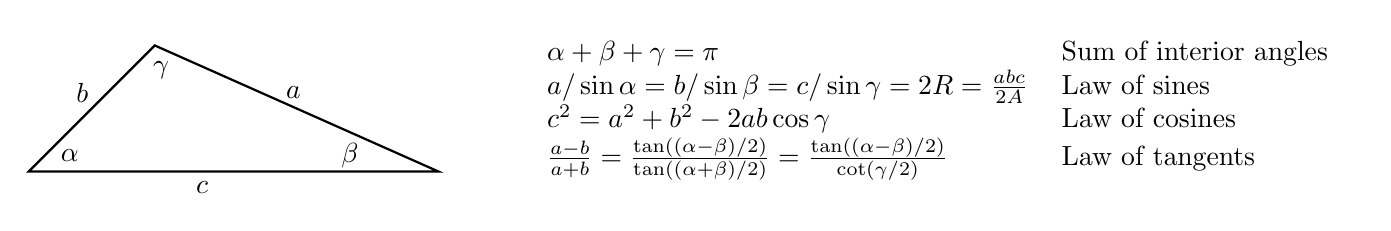
\begin{tikzpicture}[thick, scale=0.4]
\draw (0,0)--(13,0)--(4,4)--cycle;
\node at ( 1.3, 0.5) {$\alpha$};
\node at (10.2, 0.5) {$\beta$};
\node at ( 4.2, 3.2) {$\gamma$};
\node at ( 5.5,-0.5) {$c$};
\node at ( 1.7, 2.5) {$b$};
\node at ( 8.4, 2.5) {$a$};
%\node[align=left] at (17,3) {$c^2=a^2+b^2$\\ $b^2=p^2+h^2$ \\ $a^2=q^2+h^2$};
\node[align=left] at (29,2) 
{
\begin{tabular}{l l}
  $\alpha + \beta + \gamma = \pi$                       & Sum of interior angles \\
  $a / \sin \alpha = b / \sin \beta 
    = c / \sin \gamma 
    = 2R = \frac{abc}{2 A}$                             & Law of sines \\  
  $c^2 = a^2 + b^2 - 2ab \cos \gamma$                   & Law of cosines \\
  $\frac{a-b}{a+b} 
   = \frac{\tan((\alpha-\beta)/2)}{\tan ((\alpha+\beta)/2)} 
   = \frac{\tan((\alpha-\beta)/2)}{\cot (\gamma/2)}$
                                                        & Law of tangents \\
\end{tabular}
};
\end{tikzpicture}
\medskip

%\medskip
%\begin{tabular}{l l}
%  $\alpha + \beta + \gamma = \pi$                       & Sum of interior angles \\
%  $a / \sin \alpha = b / \sin \beta 
%    = c / \sin \gamma 
%    = 2R = \frac{abc}{2 A}$                             & Law of sines \\  
%  $c^2 = a^2 + b^2 - 2ab \cos \gamma$                   & Law of cosines \\
%  $\frac{a-b}{a+b} 
%   = \frac{\tan((\alpha-\beta)/2)}{\tan ((\alpha+\beta)/2)} 
%   = \frac{\tan((\alpha-\beta)/2)}{\cot (\gamma/2)}$
%                                                        & Law of tangents \\
%\end{tabular}
%\medskip
% maybe try to draw a triangle next to to the table showing all the quantities...without taking any more vertical space ...it doesn't seem to work - maybe do it in the same way as with the right triangle - include the formulas into the tikz picture - use two columns of text
% OK - done...the commented tabular environment is now inside the tikzpicture


where the quantities $R, A$ appear. These and others can be computed via:

\medskip
\begin{tabular}{l l}
 $s = (a+b+c)/2$                       & Semiperimeter, half of the perimeter \\
 $A = \sqrt{(s-a)(s-b)(s-c) s} = r s$  & Area (via Heron's formula) \\
 $r = \sqrt{(s-a)(s-b)(s-c)/s} = A/s$  & Radius of inscribed circle \\  
 $R = (abc)/ A$                        & Radius of circumscribed circle \\
 $r = \frac{s-a}{\cot(\alpha/2)}
    = \frac{s-b}{\cot(\beta/2)}
    = \frac{s-c}{\cot(\gamma/2)}$      & Law of cotangents\\
\end{tabular}
\medskip

More formulas:

\medskip
\begin{tabular}{l l}
 $\sin(\gamma / 2) = \sqrt{ (s-a)(s-b) / (a b)  }$      & Half-angle formula for sine \\
 $\cos(\gamma / 2) = \sqrt{ s(s-c) / (a b)  }$          & Half-angle formula for cosine \\
 $\tan( \gamma) = \frac{c \sin \alpha}{b - c \cos \alpha}
              = \frac{c \sin \beta} {a - c \cos \beta}$ & Tangent formula  \\
 $\frac{a-b}{c} 
   = \frac{\sin( (\alpha - \beta)/2) } { \sin( (\alpha + \beta)/2) }
   = \frac{\sin( (\alpha - \beta)/2) } { \cos( \gamma/2) } $
                                                        & Mollweide formula for sine \\
 $\frac{a+b}{c} 
 = \frac{\cos( (\alpha - \beta)/2) } { \cos( (\alpha + \beta)/2) }
 = \frac{\cos( (\alpha - \beta)/2) } { \sin( \gamma/2) } $
                                                        & Mollweide formula for cosine \\
 $c = a \cos \beta + b \cos \alpha$                     & Projection theorem \\  
 $H_a = b \sin \gamma = c \sin \beta$                   & Height above side $a$ \\ 
 $A = a H_a / 2$                                        & Area via height \\
 $M_c = \sqrt{2(a^2+b^2) - c^2}/2
      = \sqrt{a^2+b^2 +2ab\cos\gamma}/2$                & Length of median of side $c$ \\
 $B_{\gamma} = (2ab\cos(\gamma/2))/(a+b)
      = \sqrt{ab \; ((a+b)^2-c^2)}/(a+b)$               & Length of angle bisector of $\gamma$
\end{tabular}
\medskip


These are quite a lot of moderately complicated formulas already (you perhaps see now why we really don't want to memorize them) and by symmetry, even more formulas can be obtained by doing the cyclic replacements: $a \rightarrow b \rightarrow c \rightarrow a$, $\alpha \rightarrow \beta \rightarrow \gamma \rightarrow \alpha$. The median of a side is the line segment that starts from the middle of that side and goes to the vertex that is opposed to that side. All 3 medians meet in a common point which is the center of gravity of the triangle. The angle bisector is a line segment resulting from drawing a line from a vertex using half of the angle there and extending it until it hits the opposing side. All 3 angle bisectors meet in a common point which is also the center of the inscribed circle of the triangle. The center of the circumscribed circle is given by the point where perpendicular line segment bisectors meet. These are lines starting at the centers of the sides in a direction perpendicular to the respective side (ToDo: is there a formula for their lengths, too? maybe draw triangle with medians, bisectors, inscribed circle, etc.).

% see Teubner tachenbuch, page 760,764
% https://de.wikipedia.org/wiki/Projektionssatz_(Dreieck)
% todo: law of cotangents, what about centers of the incircle and circumcircle? but maybe that's for analytic geometry because it involves coordinates

\subsubsection{Congruence Theorems}
In geometry, two shapes are said to be congruent if they can be brought into full agreement just by means of translations, rotations and reflections - fancy terms for moving, turning and mirroring. It captures the idea that the two shapes are the same, just possibly placed somwhere else in space with a possibly different orientation. There are 5 theorems that state sufficient conditions for two triangles to be congruent. Two triangles are congruent if at least one of the following statements holds true: (SSS) all three sides have matching lengths, (ASA) one side and the two adjacent angles match, (SAS) one angle and the two adjacent sides match, (AAS) two angles and one side match, (SsA) two sides and the angle adjacent to the smaller side match (the lowercase 2nd s is not a typo - it indicates the smaller side). ...ToDo: verify these, especially SsA and give the algorithms to compute the missing pieces. Explain also similarity (here, also scaling is allowed - its should preserve only distance ratios where congruence preserves distances themselves. I think it also preserves angles)

% on (SsA): https://www.jstor.org/stable/27966706

%https://tutors.com/math-tutors/geometry-help/triangle-congruence-theorems-sss-sas-asa
%https://j-tradition.com/congruence.html


\subsubsection{Right Triangles}
Of special importance are triangles in which one angle is a right angle. These are unsurprisingly and rightfully called right triangles. There can be only one right angle in a non-degenerate triangle because two right angles already sum up to a straight angle, which is also the sum of all 3 angles - so if you attempt to have two right angles, you'll get a degenerate triangle whose 3rd vertex is at infinity with an angle of zero. By the way, triangles in which two sides have the same length are called isosceles and those where all three sides are equal are called equilateral. But this is just more jargon and not super important. The right triangles are the mathematically important ones. Pictured below is a right triangle with sides $a,b,c$ that is split into two further right triangles by a drawing a perpendicular from the top vertex to the base side $c$. The height of the triangle is denoted by $h$. Next to it are some relevant formulas that hold in such a situation.

\medskip
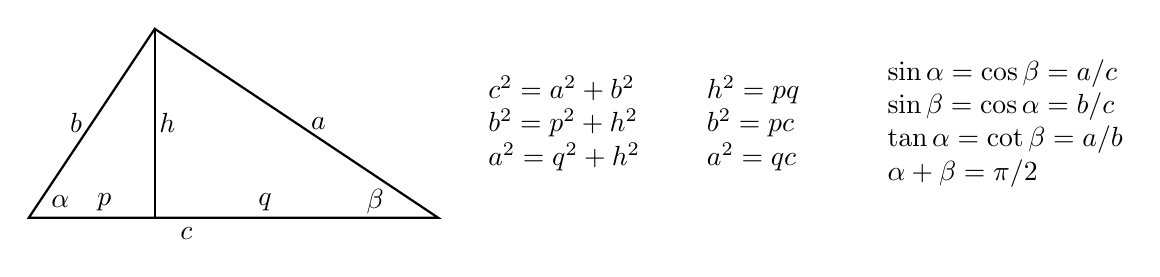
\begin{tikzpicture}[thick, scale=0.4]
\draw (0,0)--(13,0)--(4,6)--cycle;
\draw (4,6)--(4,0);
\node at (1.0, 0.5) {$\alpha$};
\node at (2.4, 0.5) {$p$};
\node at (7.5, 0.5) {$q$};
\node at (11.0, 0.5) {$\beta$};
\node at (5.0,-0.5) {$c$};
\node at (1.5,3.0)  {$b$};
\node at (9.2,3.0)  {$a$};
\node at (4.4,3.0)  {$h$};
\node[align=left] at (17,3) {$c^2=a^2+b^2$\\ $b^2=p^2+h^2$ \\ $a^2=q^2+h^2$};
\node[align=left] at (23,3) {$h^2 = p q$ \\ $b^2 = p c$ \\ $a^2 = q c$};
\node[align=left] at (31,3) {$\sin \alpha = \cos \beta = a/c$ \\ 
   $\sin \beta = \cos \alpha = b/c$ \\ 
   $\tan \alpha = \cot \beta = a/b$ \\ 
   $\alpha + \beta = \pi/2$};
\end{tikzpicture}
\medskip
% see Teubner Taschenbuch, page 761
% see at around 19:40 - Inverser Satz des Pythagoras: 1/a^2 + 1/b^2 = 1/h^2
% https://www.youtube.com/watch?v=od9lUVypXrQ


The $a^2 + b^2 = c^2$ relation is the famous theorem of Pythagoras which is a special case of the law of cosines when the angle $\gamma$ is a right angle in which case the cosine term vanishes ($\gamma$ is not shown - it's the angle opposite to side $c$). The two equations below are the same theorem applied to the sub-triangles. In the middle column are Euclid's altitude theorem (aka height theorem) and below are his theorems of sides. In the right column are some angle relations. [ToDo:verify everything, especially the $\cot \beta$ relation - it's just a guess from symmetry, maybe add also the converse relation for b/a] 

% https://tex.stackexchange.com/questions/29233/tikz-adding-text


%\begin{tikzpicture}[thick, scale=0.75]
%\draw (0,0) coordinate[label=below:$A$] (a) --
%      (4,0) coordinate[label=below:$B$] (b) --
%      (4,3) coordinate[label=above:$C$] (c) -- cycle;
%\end{tikzpicture}

%\include{Tikz/RightTriangle_4_3} % doesn't work - includes can't be nested - that sucks!!!

\subsubsection{More Triangle Facts}
% https://texample.net/tikz/examples/morleys-triangle/ trisectors always from an equilateral triangle

% there is a circle going through all of the 3 vertices - this is called the circumcircle and its center is called the crucumcentre

% each triangle has 3 "altitudes" (lines from one vertex going down orthogonally to its opposing side). They meet in a common point called the "Orthocentre"
% see: https://www.youtube.com/watch?v=ZrjarkXS0Fo

\subsection{Quadrilaterals}
% rant about why they are not called quadrangles or triangles not trilaterals

% see: https://www.youtube.com/watch?v=ZrjarkXS0Fo at 6:00
% -opposite angles in a cyclic quadrilateral sum to 180°  -and vice versa: if two opposite angles in a quadrilateral sum to 180, then the quadrilateral is cyclic (meaning that its 4 vertices lie on a circle) ..shouldn't that be called "circular" rather than "cyclic"

% Ptolemy’s Theorem and the Almagest: we just found the best visual proof in 2000 years
% https://www.youtube.com/watch?v=rr1fzjvqztY
% In any cyclic quadrilateral (i.e. qudrilatral inscribed in a circle). Label 2 opposite sides A,a and the tow other opposite sides B,b and the two diagonals C,c. Then: A*a + B*b = C*c. If the quadrilateral is a rectangle, we recover Pythogoras's theorem a special case.

\subsection{Polygons}
% sums of interior and exterior angles

\subsection{Circles}

% https://www.youtube.com/watch?v=rr1fzjvqztY
% 6:20: start with any chord of the circle. from the ends of the chord, draw lines that meet at the circle. all pairs of such lines will meet in the same angle at the circle
% if you also draw lines to the center of the circle, the meeting angle at the center is twice that of the meeting angle at the boundary
% when the chord goes through the center, the meeting angles at the circle's boudary are 90° (Thales theorem)

% https://en.wikipedia.org/wiki/N-sphere#Spherical_coordinates

\subsection{Geometric Derivations}
You may wonder, how all these formulas were derived geometrically or how one would go about deriving a formula geometrically at all. The process starts with a couple of points, lines or line segments and maybe circles and then makes use of the Euclidean axioms: we may pick any pair of points and draw a line between them, we may extend lines as we see fit, we may draw a circle centered at one of our points with a radius given by the distance between any pair of our points. In such a construction, we may then identify angles that must be equal to each other by the rules of corresponding, opposite, alternating or consecutive angles. We may identify sums of angles that must sum up to a right, straight or full angle. We may identify line segments or distance ratios that must be equal to each other. We may identify shapes that are congruent or similar to one another. All of that will give us equations. What exactly to do in a given situation to find such equations is a highly creative process. Look up "Dandelin Spheres" or watch 3blue1brown's "Why slicing a cone gives an ellipse" video for a nice example of such a geometric proof. A much simpler example is the proof that the sum of all angles in a triangle must be a straight angle...

% https://www.youtube.com/watch?v=pQa_tWZmlGs
% https://en.wikipedia.org/wiki/Dandelin_spheres

ToDo: draw the picture that shows that the angles in a triangle must sum to 180

\begin{comment}
	
Maybe explain why we say triangles and quadrilaterals but not, more consistently, either triangles and quadrangles or trilaterals and quadrilaterals. One suffix-term focuses on the angles, the other on the sides - I think

https://texample.net/tikz/examples/area/geometry/
http://www.tikzedt.org/

https://github.com/walmes/Tikz  examples mainly for statistics

-center circumscribed circle: intersection of medians
-center of inscribed circle: intersection of angle bisectors

https://en.wikipedia.org/wiki/Median_(geometry)
https://de.wikipedia.org/wiki/Seitenhalbierende

https://mathworld.wolfram.com/AngleBisector.html
https://en.wikipedia.org/wiki/Angle_bisector_theorem
https://en.wikipedia.org/wiki/Bisection#Triangle
https://de.wikipedia.org/wiki/Winkelhalbierende

https://mathworld.wolfram.com/PerpendicularBisector.html
https://en.wikipedia.org/wiki/Bisection#Perpendicular_line_segment_bisector
https://de.wikipedia.org/wiki/Mittelsenkrechte

https://en.wikipedia.org/wiki/Incircle_and_excircles_of_a_triangle

https://en.wikipedia.org/wiki/Mollweide%27s_formula

https://en.wikipedia.org/wiki/Law_of_cotangents

https://en.wikipedia.org/wiki/Circle

-thales' theorem

-rename file to Geo_Elementary

-plot a drawing of a triangle with vertices A,B,C, sides a,b,c and angles alpha, beta, gamma
-give a bunch of formulas that hold for all triangles
-the plot some special triangles (right, isosceles, etc.) and give the formulas specific to them
-mention non-Euclidean trigonometry, espeically spherical...maybe give the formulas for those
triangles, too - or maybe refer to some ressource

-give formulas for volumes of 3D shapes

https://en.wikipedia.org/wiki/Trigonometry

Weitz: Elementargeometrie (Vorkurs Mathematik)
https://www.youtube.com/watch?v=cMuoFr4DvDo

Weitz: Überblick Elementargeometrie: Winkel, Satz des Pythagoras, Sinus, Kosinus, etc.
https://www.youtube.com/watch?v=zVLFfgg7f98&list=PLb0zKSynM2PBYzz6l37rWH3B_n_7P40QP&index=167

How many lines go through 4 given lines in 3D?
https://www.youtube.com/watch?v=F5d8fUXf7d8
-6:40 Galucci's Theorem: 3 skew lines in 3D always define a ruling of either hyperboloid 
 or (in exceptional cases when all 3 lines are parallel to the same plane) a hyperbolic 
 paraboloid (see also: ruled surface). 
-A hyperboloid has two different rulings. A line from one such ruling intersects all lines of the
 other ruling. 
-This implies that for 3 given lines in 3D, there are infinitely many lines that intersect all 3.
-For 4 given lines on 3D, there are 4 cases: 
 1: the 4th line does not intersect the hyperboloid -> no line exists that intersects all 4
 2: the 4th line is tangent to the hyperboloid -> one line intersects all 4
 3: the 4th line pokes through the hyperboloid -> two lines intersect all 4
 4: the 4th lines lies on the same ruling of the hyperboloid -> infinitely many lines intersect 
    all 4 (namely, those on the opposite ruling)
-This is a topic of enumerative geometry and Schubert Calculus

the forgotten 3 dimensional Pythagorean theorem.
https://www.youtube.com/watch?v=vcnQ0GR4IPI
https://en.wikipedia.org/wiki/De_Gua%27s_theorem

Divine high PHI: The power of AB=A+B (Mathologer masterclass)
https://www.youtube.com/watch?v=cCXRUHUgvLI
at 6:40 - Ptolemys theorem - generalization of Pythagoras theorem


\end{comment}